\frame[plain]{\titlepage}
\frame{\frametitle{Outline}\tableofcontents}

\section{Problem - Nonlinear Real Arithmetic}
\subsection{Syntax of SMT(NRA)}

\begin{frame}
    \frametitle{Syntax of SMT(NRA)}
    
    polynomial: $p ::= x \mid c \mid p + p \mid p - p \mid p \times p$

    atoms: $a ::= b \mid p = 0 \mid p > 0 \mid p < 0$

    formula: $f ::= a \mid \neg f \mid f \wedge f \mid f \vee f $

    \vspace{0.4cm}

    SMT: Determine whether the formula is satisfied by some assignment (local search focuses), or prove unsat

    \vspace{0.4cm}

    Example:
    \\
    $x^2 + y^2 \le 1 \wedge x + y < 1 \wedge x + z > 0$
    \\
    assignment with $\left\{x \rightarrow 0, y \rightarrow 0, z \rightarrow 1\right\}$ satisfies all clauses.
\end{frame}

\begin{frame}{Fragment of Local Search (1)}
    \begin{algorithm}[H]
    \SetKwBlock{Begin}{}{}
    \SetAlgoLined
    \SetKwInOut{Input}{Input}
\SetKwInOut{Output}{Output}
\Input{A set of clauses $F$}
\Output{An assignment satisfying $F$, or failure}
Initialize assignment to variables\;
\While{$\top$}{
    \If{all clauses satisfied}{
        \Return{success with assignment\;}
    }
    \If{time or step limit reached}{
        \Return{failure\;}
    }
    Critical move procedure.
}
    \caption{Basic Fragment of Local Search\footfullcite{CaiLZ22}}
    \end{algorithm}
\end{frame}

\begin{frame}{Fragment of Local Search (2)}
    \begin{algorithm}[H]
    \SetKwBlock{Begin}{}{}
    \begin{minipage}{0.45\textwidth}
        \caption{First Part of the Algorithm}
        $\mathit{var,new\_value,score} \leftarrow$ best move according to make-break score\;
    \If{score $>$ 0}{
        Move $\mathit{var}$ to $\mathit{new\_value}$\;
    }
    \Else{
        Update clause weight\;
    }
    \end{minipage}
    \hfill
    \begin{minipage}{0.45\textwidth}
        \caption{Second Part of the Algorithm}
        \Repeat{3 times}{
            $\mathit{cls} \leftarrow$ random unsatisfied clause\;
            $\mathit{var,new\_value,score} \leftarrow$ critical move making $\mathit{cls}$ satisfied\;
            \If{score $\neq$ $-\infty$}{
                move $\mathit{var}$ to $\mathit{new\_value}$\;
            }
        }
        \If{no move performed}{
            Move some variables in unsatisfied clauses\;
        }
    \end{minipage}
    \end{algorithm}
\end{frame}
    

\begin{frame}
    \frametitle{Local Search for SAT and SMT}

    \begin{center}
        \begin{tabular}{|c|c|c|}
            \hline
            \diagbox{LS}{Problem}&SAT&SMT\\
            \hline
            Operation (Move)&Flip&Critical Move\\
            \hline
            Score Definition & \multicolumn{2}{c|}{Weighted unsat clauses}\\
            \hline
            Score Computation & Cached score& No Caching, time costly\\
            \hline 
            \end{tabular}
    \end{center}

    \textbf{What LS for SAT brings us: }\\
    Maintain scoring information after each iteration.\\
    \textbf{Difficulty:}\\
    Predetermine critical move shift value.\\
    \textbf{Our Solution:}\\
    Introduce Scoring Boundaries.
\end{frame}

\subsection{Fragment of Local Search}

\section{Incremental Computation of Variable Scores}
\subsection{Scoring Boundary for Arithmetic Variable}

\begin{frame}{Infeasible Set}
    \begin{definition}
        \textbf{infeasible set\footfullcite{JovanovicM12}} of a clause $c$ with respect to an assignment $\mathit{asgn}$ is the set of values that the variables in $c$ can take under $\mathit{asgn}$ such that $c$ is unsatisfied.
    \end{definition}
    \begin{example}
        Current assignment: $\left\{ x\mapsto 1\right\}$ \\
        Calculate infeasible set for $y$:
        \begin{itemize}
            \item $x^2+y^2\le 1$ : $(-\infty, 0) \cup (0, \infty)$.
            \item $x+y<1$ : $[0,\infty)$.
        \end{itemize}
    \end{example}
    If we choose values from infeasible set, the satisfied clause will be unsatisfied, which changes the whole score.
\end{frame}

\begin{frame}{Make-break Intervals}
    \begin{definition}
        \textbf{make-break interval}\footfullcite{abs-2303-06676} is a 
    combination of (in)feasible intervals of arithmetic varaible $x$ with respect to \textbf{all clauses}.
    \end{definition}

    \begin{example}
        Current assignment: $\left\{ x\mapsto 1, y\mapsto 1, z\mapsto 1 \right\}$ \\
        Calculate infeasible set for each clause.
        \begin{itemize}
            \item $x^2+y^2\le 1$ (unsat): $(-\infty, 0) \cup (0, \infty)$.
            \item $x+y<1$ (unsat): $[0,\infty)$.
            \item $x+z>0$ (sat): $(-\infty,-1]$.
        \end{itemize}
        Combined information: $x$: $(-\infty,-1]\mapsto 0$, $(-1,0)\mapsto 1$, $[0,0]\mapsto 1$, $(0,\infty)\mapsto 0$.
    \end{example}
\end{frame}

\begin{frame}{Traditional Computation}
    \begin{algorithm}[H]
        \SetKwBlock{Begin}{}{}
        \SetAlgoLined
        \SetKwInOut{Input}{Input}
    \SetKwInOut{Output}{Output}
    \Input{unsat clauses $F$}
    \Output{Best critical move (variable, value)}
    \ForEach{variable $v$ in unsat clauses}{
        \ForEach{unsat clause $c$ with $v$}{        Compute interval-score info of $v$ in $c$.
        }
        Combine interval-score information. \\
        Update best var-value move.
    }
    \Return{best critical move}
    \end{algorithm}
    
    \vspace{0.4cm}
    \textbf{Repeated computation:}\\
    \begin{itemize}
        \item variable's (in)feasible set
        \item clause's sat staus
    \end{itemize}

\end{frame}

\begin{frame} 
    \frametitle{Boundary}
    \textbf{Definition.} A quadruple $\langle \mathit{val}, \mathit{is\_open}, \mathit{is\_make}, \mathit{cid}\rangle$, where $\mathit{val}$ is a real number, $\mathit{is\_open}$ and $\mathit{is\_make}$ are boolean values, and $\mathit{cid}$ is a clause identifier.
    \vspace{0.4cm}
    \begin{alertblock}{Meaning}
        \begin{itemize}
            \item $val:$ make-break value.
            \item $is\_open:$ active or not at $val$ point.
            \item $is\_make:$ make or break, increase or decrease score.
            \item $cid:$ causing clause.
        \end{itemize}
    \end{alertblock}

    \textbf{Sorting:} First ordered by $val$, then by $is\_open$ ($\bot<\top$).
\end{frame}

\begin{frame}
    \frametitle{Boundary}
    Current assignment: $\left\{ x\mapsto 1, y\mapsto 1, z\mapsto 1 \right\}$ \\
    \begin{itemize}
        \item $x^2+y^2\le 1$: starting score 0, boundary set $\{(0,\bot,\top,1), (0,\top,\bot,1)\}$, indicating no change for large negative values, \emph{make} at boundary $[0,\cdots$, followed by \emph{break} at boundary $(0,\cdots$.
        \item $x+y<1$: starting score 1, boundary set $\{(0,\bot,\bot,1)\}$, indicating \emph{make} at large negative values, and \emph{break} at boundary $[0,\dots$.
        \item $x+z>0$: starting score $-1$, boundary set $\{(-1,\top,\top,1)\}$, indicating \emph{break} at large negative values, and \emph{make} at boundary $(-1,\dots$.
    \end{itemize}
    sorted boundary set: $\{(-1,\top,\top,1),(0,\bot,\top,1),(0,\bot,\bot,1),(0,\top,\bot,1)\}$
\end{frame}

\subsection{Incremental Computation}

\begin{frame}{Boundary Example}
    boundary set: $\{(-1,\top,\top,1),(0,\bot,\top,1),(0,\bot,\bot,1),(0,\top,\bot,1)\}$
    \vspace{0.2cm}
    \begin{center}
        \begin{tikzpicture}
            \draw[->] (-4,0)--(4,0);
            \foreach \x in {0,2}
            {
                \draw[xshift=\x cm] (-2,0) -- (-2,0.1);
            };  
            \node[below] at (0,0){0};
            \foreach \x in {-1,0} {
                \node[below] at(2 *\x,0){\x};
            }
            % starting score
            \node[below] at (-3,0.75){0};
            \node[below] at (-2,0.75){1};
            \node[below] at (0,0.75){1};
            \node[below] at (2,0.75){0};

            \node[below] at (-3,-0.5){0+1-1};
            \node[below] at (-1.75,-0.5){0+1};
            \node[below] at (0,-0.5){1+1-1};
            \node[below] at (2,-0.5){1-1};
        \end{tikzpicture}
    \end{center}

    \textbf{Starting score:} Score when $x$ moves to -$\infty$. \\
    \textbf{Maintain and Change:} We maintain the boundary info for all arithmetic varaibles, unless the neighbour does a critical move.
\end{frame}

\begin{frame}{Algorithm for computing boundary}
    \begin{algorithm}[H]
        \SetKwBlock{Begin}{}{}
        \SetAlgoLined
        \SetKwInOut{Input}{Input}
    \SetKwInOut{Output}{Output}
    \Input{Variable $v$ that is modified}
    \Output{Make-break score for all variables}
    $S \leftarrow \{\}$ \tcp*{set of updated variables}
    \For{clause $\mathit{cls}$ that contains $v$}{
        \For{variable $v'$ appearing in $\mathit{cls}$}{
            add $v'$ to $S$\;
            recompute starting score and boundary of $v'$ with respect to $\mathit{cls}$\;
        }
    }
    \For{variable $v'$ in S}{
        recompute best critical move and score in terms of boundary information\;
    }
    \end{algorithm}
\end{frame}

\section{Temporary Relaxation of Equality (Non-Strick) Constraints}

\subsection{Value Complexity in Local Search}

\begin{frame}{Complexity of Values}
    \begin{definition}
        We define a preorder $\prec_c$ on algebraic numbers as follows. $x\prec_c y$ if $x$ is rational and $y$ is irrational, or if both $x$ and $y$ are rational numbers, and the denominator of $x$ is less than that of $y$. We write $x \sim_c y$ if neither $x\prec_c y$ nor $y\prec_c x$.
    \end{definition}
    Previous work  ignores equalities constraints\footfullcite{LiXZ23}, or only consider multi-linear (one-degree)examples\footfullcite{abs-2303-06676}.\\

    \textbf{Our Solution:} Introducing relaxation, temporary enlarge the point irrational interval
\end{frame}

\subsection{Relaxation Method}
\begin{frame}{Relaxation}
    \begin{Example}
        Given assignment $\left\{x\mapsto 1, y\mapsto 1\right\}$
        \begin{minipage}{0.45\textwidth}
            \centering
            $z^2 = x^2 + y^3$
        \end{minipage}
        % \hfill
        \begin{minipage}{0.45\textwidth}
            \centering
            $z^3 \ge 5 x^2 + y \vee z^3 \le 3x + 3y$
        \end{minipage}
        \end{Example}
        \vspace{0.6cm}
        Both situations force $z$ to an irrational number.

    \begin{alertblock}{Relaxation}
    \begin{itemize}
        \item If the constraint is of the form $p=0$, it is relaxed into the pair of inequalities $p<\epsilon_p$ and $p>-\epsilon_p$.

        \item If the constraint is of the form $p\ge 0$, it is relaxed into $p>-\epsilon_p$. Likewise, if the constraint is of the form $p\le 0$, it is relaxed into $p<\epsilon_p$.
        \item \textbf{Slacked var:} the var that is being assigned.
    \end{itemize}
    \end{alertblock}
\end{frame}

\begin{frame}{Restore}
    \begin{algorithm}[H]
        \SetKwBlock{Begin}{}{}
        \SetAlgoLined
        \SetKwInOut{Input}{Input}
    \SetKwInOut{Output}{Output}
    \Input{slacked clauses}
    \Output{succeed or not}
    \For{each slacked clause $\mathit{cls}$}{
        $v \leftarrow$ slacked variable in $\mathit{cls}$\;
        $accu\_val \leftarrow inf\_set(cls)$\;
        move $v$ to $accu\_val$\;
    }
    \For{variable $v'$ in slacked clauses}{
        recompute best critical move and score in terms of boundary information\;
    }
    \Return number of unsat clauses == 0
    \end{algorithm}
\end{frame}

\begin{frame}{Local Search with Relaxation}
    \scriptsize
    \begin{algorithm}[H]
\label{alg:relax}
\SetKwInOut{Input}{Input}
\SetKwInOut{Output}{Output}
\Input{A set of clauses $F$}
\Output{An assignment of variables that satisfy $F$, or failure}
Initialize assignment to variables\; 
\While{$\top$}{
    \If{all clauses satisfied}{
        $\mathit{success} \leftarrow$ find exact solution\;
        \If{success}{
            \Return{success with assignment};
        }
        \Else{
            Restore relaxed constraints to original form\;
            $\mathit{success} \leftarrow$ find exact solution by limited local search\;
            \If{success}{
                \Return{success with assignment};
            }
        }
    }
    \If{time or step limit reached}{
        \Return{failure}\;
    }
    Proceed traditional local search (slack).
}
    \end{algorithm}
\end{frame}

\section{Experiment}

\begin{frame}{Implementation Detail}
    \textbf{code available at:} \url{https://github.com/yogurt-shadow/LS_NRA}

    \textbf{Preprocessing} 
    \begin{itemize}
        \item Combine constraints $p\ge 0$ and $p\le 0$ into equality $p=0$.
        \item Eliminate variable $x$ in an equation of the form $c\cdot x+q=0$, where $c$ is a constant and $q$ is a polynomial with degree at most 1 and containing at most 2 variables.
    \end{itemize}

    \textbf{Restart mechanism} Two-level restart mechanism with two parameters $T_1 = 100$ and $T_2 = 100$.

    \begin{itemize}
        \item \textbf{Minor restart:} randomly change one of the variables in one of the unsatisfied clauses.
        \item \textbf{Major restart:} reset the value of all variables.
    \end{itemize}
\end{frame}

\begin{frame}{Overall Result}
    \begin{table}[!t]
        \centering
        \small
        \begin{tabular}{c | c | c | c | c | c | c}
                    Category & \#inst & Z3 & cvc5 & Yices & ~Ours~ & ~Unique~ \\ \hline
                    20161105-Sturm-MBO & 120 & 0 & 0 & 0 & \textbf{88} & 88 \\
                    20161105-Sturm-MGC & 2 & \textbf{2} & 0 & 0 & 0 & 0 \\
                    20170501-Heizmann & 60 & 3 & 1 & 0 & \textbf{8} & 6 \\
                    20180501-Economics-Mulligan & 93 & \textbf{93} & 89 & 91 & 90 & 0 \\
                    2019-ezsmt & 61 & \textbf{54} & 51 & 52 & 19 & 0 \\
                    20200911-Pine & 237 & \textbf{235} & 201 & \textbf{235} & 224 & 0 \\
                    20211101-Geogebra & 112 & \textbf{109} & 91 & 99 & 101 & 0 \\
                    20220314-Uncu & 74 & 73 & 66 & \textbf{74} & 70 & 0 \\
                    LassoRanker & 351 & 155 & \textbf{304} & 122 & 272 & 13\\
                    UltimateAtomizer & 48 & \textbf{41} & 34 & 39 & 27 & 2 \\
                    hycomp & 492 & \textbf{311} & 216 & 227 & 304 & 11 \\
                    kissing & 42 & \textbf{33} & 17 & 10 & \textbf{33} & 1 \\
                    meti-tarski & 4391 & \textbf{4391} & 4345 & 4369 & 4351 & 0 \\
                    zankl & 133 & 70 & 61 & 58 & \textbf{100} & 27 \\ \hline
                    Total & 6216 & 5570 & 5476 & 5376 & \textbf{5687} & 148 
                \end{tabular}
        % \bottomrule
        % \multicolumn{4}{l}{\small $\bullet$ Solved by ours.}\\
        \end{table}
\end{frame}

\begin{frame}{Scatter Plot}
    \begin{figure}
        \centering
        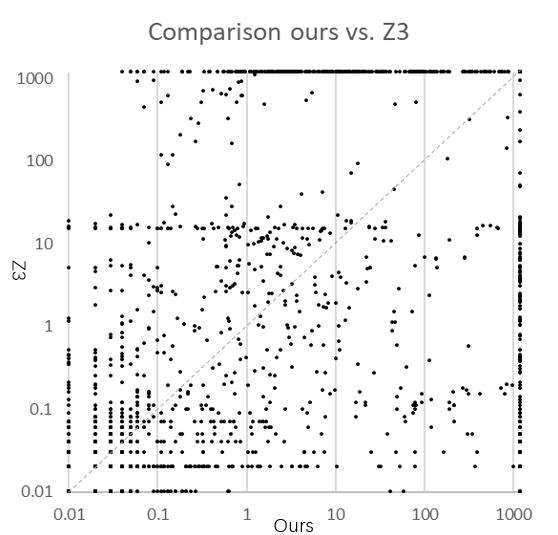
\includegraphics[width=0.45\textwidth]{scatter_z3b.png}\qquad
        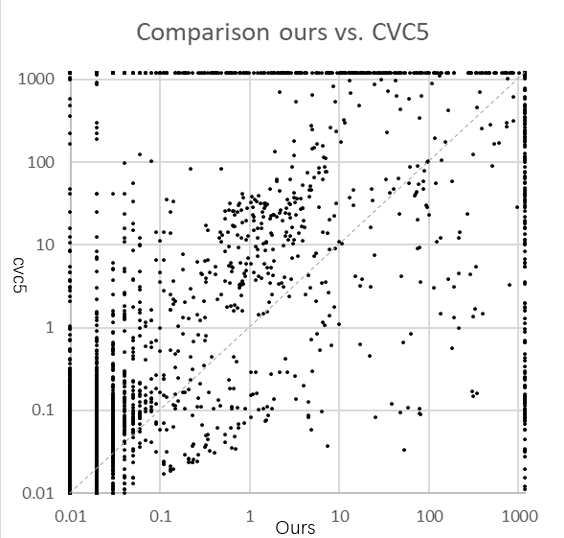
\includegraphics[width=0.45\textwidth]{scatter_cvc5b.png}
        \caption{Scatter plots of running time vs. Z3 and cvc5.}
        \label{fig:scatter_plots}
    \end{figure}
\end{frame}

\begin{frame}
    \begin{table}[!t]
        \small
        \centering
        \begin{tabular}{c | c | c | c | c }
        Category & ~\#inst~ & ~Incremental~ & ~Naive~ & ~Limit-45~ \\ \hline
        20161105-Sturm-MBO & 120 & 88 & 85 & 85 \\
        20161105-Sturm-MGC & 2 & 0 & 0 & 0 \\
        20170501-Heizmann & 60 & 8 & 5 & 5 \\
        20180501-Economics-Mulligan & 93 & 90 & 89 & 89 \\
        2019-ezsmt & 61 & 19 & 19 & 15 \\
        20200911-Pine & 237 & 224 & 222 & 222 \\
        20211101-Geogebra & 112 & 101 & 101 & 101 \\
        20220314-Uncu & 74 & 70 & 70 & 70 \\
        LassoRanker & 351 & 272 & 264 & 269 \\
        UltimateAtomizer & 48 & 27 & 26 & 26 \\
        hycomp & 492 & 304 & 298 & 298 \\
        kissing & 42 & 33 & 32 & 33 \\
        meti-tarski & 4391 & 4351 & 4352 & 4352 \\
        zankl & 133 & 100 & 100 & 100 \\ \hline
        Total & 6216 & 5687 & 5663 & 5665
        \end{tabular}
        \vspace{2mm}
        \caption{Comparison of incremental computation}
        \label{tab:compare-incremental}
        \end{table}
\end{frame}

\begin{frame}
    \begin{table}[!t]
        \small
        \centering
        \begin{tabular}{c | c | c | c | c }
        Category & ~\#inst~ & ~Relaxation~ & ~Threshold~ & ~NoOrder~ \\ \hline
        20161105-Sturm-MBO & 120 & 88 & 100 & 99 \\
        20161105-Sturm-MGC & 2 & 0 & 0 & 0 \\
        20170501-Heizmann & 60 & 8 & 9 & 3 \\
        20180501-Economics-Mulligan & 93 & 90 & 89 & 86 \\
        2019-ezsmt & 61 & 19 & 19 & 19 \\
        20200911-Pine & 237 & 224 & 223 & 222 \\
        20211101-Geogebra & 112 & 101 & 98 & 92 \\
        20220314-Uncu & 74 & 70 & 70 & 70 \\
        LassoRanker & 351 & 272 & 277 & 278 \\
        UltimateAtomizer & 48 & 27 & 26 & 20 \\
        hycomp & 492 & 304 & 211 & 164 \\
        kissing & 42 & 33 & 31 & 27 \\
        meti-tarski & 4391 & 4351 & 4353 & 4360 \\
        zankl & 133 & 100 & 100 & 100 \\ \hline
        Total & 6216 & 5687 & 5606 & 5540
        \end{tabular}
        \vspace{2mm}
        \caption{Comparison of temporary relaxation of constraints}
        \label{tab:compare-relaxation}
        \end{table}
\end{frame}

\begin{frame}{Future Work}
    \begin{itemize}
        \item Integrate into z3++ solver \url{https://z3-plus-plus.github.io/}
        \item Cacheing about cylindrical cells by CAD (we enter the same cell multiple times, how can we find that?)
        \item incorporate with other algorithms, like MCSAT or varaible substitution.
        \item used for nonlinear optimization
    \end{itemize}
\end{frame}

\begin{frame}[allowframebreaks]
    \frametitle{References}
\printbibliography
\end{frame}